\subsection{装饰器模式(Decorator)}

\subsubsection{装饰器模式简介}


装饰器模式是一种常用的设计模式。它可以在不更改原有对象的基础上,通过组合的方式为对象添加新的功能。装饰器模式通过创建一个装饰类,并将原有对象作为装饰类的一个属性,来实现对原有对象的功能扩展。

例如,在游戏中,可能会有一个基础的人物类,该类可以描述人物的基本信息和属性。如果我们想为人物添加新的能力,例如飞行能力,就可以使用装饰器模式。我们可以创建一个装饰类,将人物类作为该装饰类的一个属性,并在装饰类中定义飞行能力的相关方法。这样,我们就可以在不更改原有人物类的基础上,为人物添加飞行能力。

\subsubsection{装饰器模式在项目中的应用}

\begin{figure}[h]
  \centering
  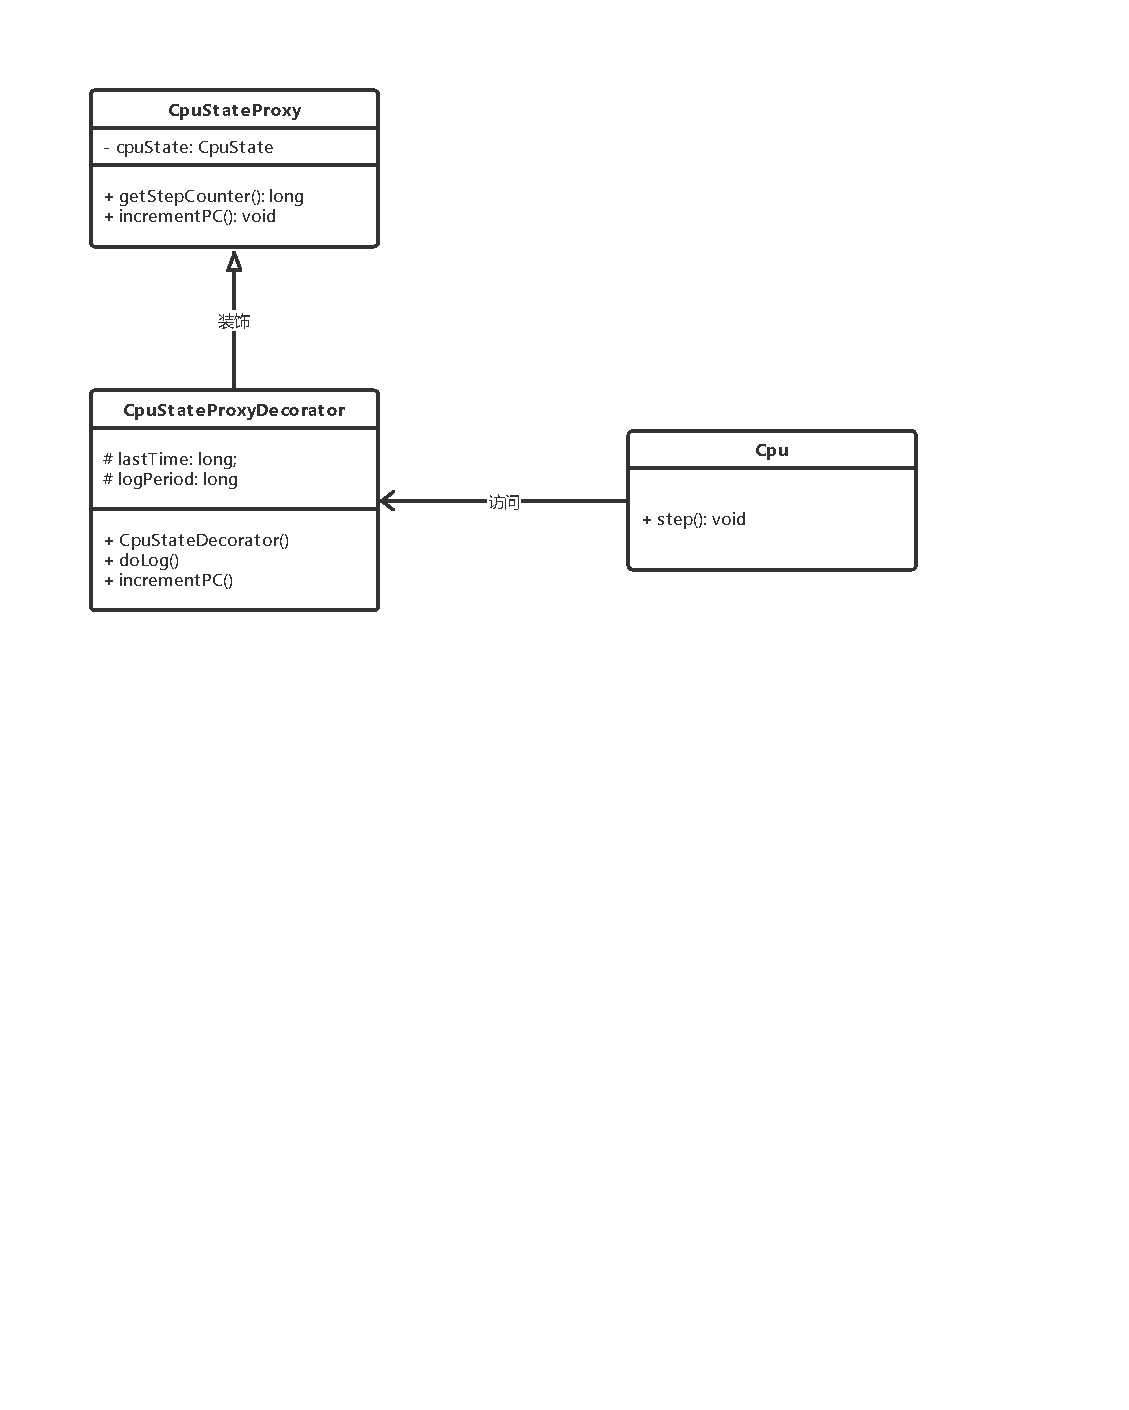
\includegraphics[width=0.9\textwidth]{figures/装饰器模式.pdf}
  \caption{装饰器模式在 Slow6502 中的类图}
\end{figure}

在我们的项目中,我们使用装饰器模式使一些类能够记录相关的日志。使用装饰器模式来实现日志记录是十分自然的。装饰器模式可以在不更改原有对象的基础上,为对象添加新的功能。因此,我们可以通过创建一个装饰类,并将需要记录日志的类作为该装饰类的一个属性,来实现日志记录的功能。这样,我们就可以在不更改原有类的基础上,为这些类添加日志记录的能力。

另外,使用装饰器模式实现日志记录还可以提高代码的可维护性。当我们需要更改日志记录的方式时,只需要更改装饰类的实现,而不需要更改原有的类。这样可以避免对原有类的修改,提高代码的可维护性。